\documentclass[tikz, border=10pt]{standalone}
\usepackage{tikz}
\usepackage{amsmath}
\usetikzlibrary{shapes, calc, backgrounds}

% Slide version of figures/voronoi_vertical_stack.tex, drawn at the exact
% coordinates of the proof of the strict-separation theorem (Appendix A):
%   p_C = (0.8, 0.1, 0.1), p_A = (0.4, 0.3, 0.3), p_B = (0, 0.5, 0.5),
%   mu_0 = e_0, mu_1 = (0.4, 0.5, 0.1), mu_2 = (0.1, 0.4, 0.5).
% A simplex point p maps to p_0 * Top + p_1 * Right + p_2 * Left.
\begin{document}
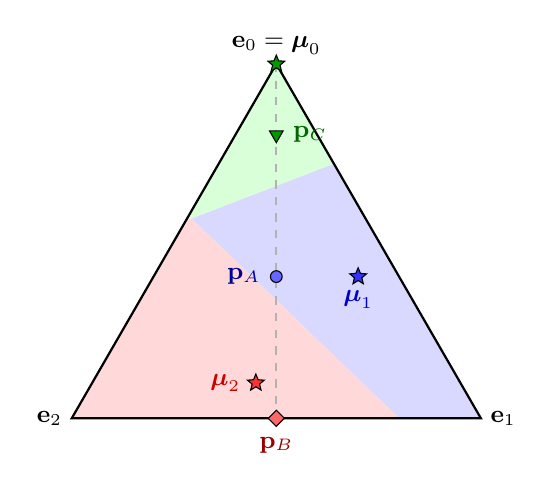
\begin{tikzpicture}[scale=0.6, font=\sffamily]

    % Simplex vertices.
    \coordinate (Top) at (0, 5);
    \coordinate (Right) at (4.33, -2.5);
    \coordinate (Left) at (-4.33, -2.5);

    % Prototypes.
    \coordinate (Mu0) at (0, 5);
    \coordinate (Mu1) at (1.732, 0.5);
    \coordinate (Mu2) at (-0.433, -1.75);

    % Data points on the altitude p_1 = p_2.
    \coordinate (C) at (0, 3.5);
    \coordinate (A) at (0, 0.5);
    \coordinate (B) at (0, -2.5);

    % Voronoi cells, each clipped to the simplex and to two half-planes.
    \begin{scope}
        \clip (Top) -- (Right) -- (Left) -- cycle;
        \path (Mu0) -- (Mu1) coordinate[midway] (M01);
        \clip ($(M01)!20cm!90:(Mu1)$) -- ($(M01)!20cm!-90:(Mu1)$) -- ($(M01)!20cm!180:(Mu1)$) -- cycle;
        \path (Mu0) -- (Mu2) coordinate[midway] (M02);
        \clip ($(M02)!20cm!90:(Mu2)$) -- ($(M02)!20cm!-90:(Mu2)$) -- ($(M02)!20cm!180:(Mu2)$) -- cycle;
        \fill[green!15] (-5,-5) rectangle (5,6);
    \end{scope}

    \begin{scope}
        \clip (Top) -- (Right) -- (Left) -- cycle;
        \path (Mu1) -- (Mu0) coordinate[midway] (M10);
        \clip ($(M10)!20cm!90:(Mu0)$) -- ($(M10)!20cm!-90:(Mu0)$) -- ($(M10)!20cm!180:(Mu0)$) -- cycle;
        \path (Mu1) -- (Mu2) coordinate[midway] (M12);
        \clip ($(M12)!20cm!90:(Mu2)$) -- ($(M12)!20cm!-90:(Mu2)$) -- ($(M12)!20cm!180:(Mu2)$) -- cycle;
        \fill[blue!15] (-5,-5) rectangle (5,6);
    \end{scope}

    \begin{scope}
        \clip (Top) -- (Right) -- (Left) -- cycle;
        \path (Mu2) -- (Mu0) coordinate[midway] (M20);
        \clip ($(M20)!20cm!90:(Mu0)$) -- ($(M20)!20cm!-90:(Mu0)$) -- ($(M20)!20cm!180:(Mu0)$) -- cycle;
        \path (Mu2) -- (Mu1) coordinate[midway] (M21);
        \clip ($(M21)!20cm!90:(Mu1)$) -- ($(M21)!20cm!-90:(Mu1)$) -- ($(M21)!20cm!180:(Mu1)$) -- cycle;
        \fill[red!15] (-5,-5) rectangle (5,6);
    \end{scope}

    % Simplex frame and the altitude p_1 = p_2.
    \draw[thick] (Top) -- (Right) -- (Left) -- cycle;
    \draw[dashed, gray!60, thick] (0, 5) -- (0, -2.5);

    \node[above, font=\small] at (Top) {$\mathbf{e}_0 = \boldsymbol{\mu}_0$};
    \node[right, font=\small] at (Right) {$\mathbf{e}_1$};
    \node[left, font=\small] at (Left) {$\mathbf{e}_2$};

    % Prototypes (stars).
    \node[star, star points=5, star point ratio=2.25, fill=green!60!black, draw=black, inner sep=1pt] at (Mu0) {};

    \node[star, star points=5, star point ratio=2.25, fill=blue!80, draw=black, inner sep=1pt] (Star1) at (Mu1) {};
    \node[below, blue!80!black, font=\small\bfseries] at (Star1.south) {$\boldsymbol{\mu}_1$};

    \node[star, star points=5, star point ratio=2.25, fill=red!80, draw=black, inner sep=1pt] (Star2) at (Mu2) {};
    \node[left, red!80!black, font=\small\bfseries] at (Star2.west) {$\boldsymbol{\mu}_2$};

    % Data points, labelled with their true class.
    \node[regular polygon, regular polygon sides=3, rotate=180, fill=green!60!black, draw=black, inner sep=1pt] (NodeC) at (C) {};
    \node[right, green!40!black, font=\small\bfseries] at ($(C)+(0.15,0)$) {$\mathbf{p}_C$};

    \node[circle, fill=blue!60, draw=black, inner sep=1.5pt] (NodeA) at (A) {};
    \node[left, blue!60!black, font=\small\bfseries] at (NodeA.west) {$\mathbf{p}_A$};

    \node[diamond, fill=red!60, draw=black, inner sep=1.5pt] (NodeB) at (B) {};
    \node[below, red!60!black, font=\small\bfseries] at (NodeB.south) {$\mathbf{p}_B$};

\end{tikzpicture}
\end{document}
